\documentclass[parskip]{scrartcl}

\usepackage{pgfplots}

\subject{Sheet 02}
\title{PS Parallel Programming}
\author{Patrick Wintner}
\date{\today}

\begin{document}
	\maketitle
	
	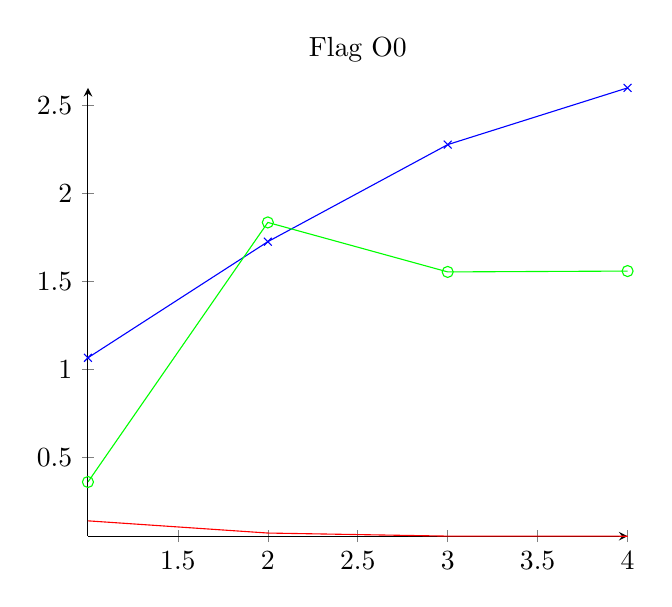
\begin{tikzpicture}
		%flag O0
		\begin{axis}[axis x line=middle, axis y line=center, title={Flag O0}]
			\addplot[color=blue,mark=x] coordinates {
				(1,1.067867) (2,1.727467) (3,2.279000) (4,2.601400) % slow
			};		
			\addplot[color=green,mark=o] coordinates {
				(1,0.362133) (2, 1.836900) (3, 1.555700) (4, 1.560533) % medium
			};
			\addplot[color=red] coordinates {
				(1, 0.141433) (2, 0.072100) (3, 0.054600) (4, 0.054167) % fast
			};
		\end{axis}
	\end{tikzpicture}
	
	\begin{tikzpicture}
	%flag O1
		\begin{axis}[axis x line=middle, axis y line=center, title={Flag O1}]
			\addplot[color=blue,mark=x] coordinates {
				(1,1.061733) (2,1.703600) (3,1.950833) (4,2.347333) % slow
			};		
			\addplot[color=green,mark=o] coordinates {
				(1,0.359967) (2, 1.942000) (3, 1.839400) (4, 1.793233) % medium
			};
			\addplot[color=red] coordinates {
				(1, 0.020700) (2, 0.013433) (3, 0.013233) (4, 0.011600) % fast
			};
		\end{axis}
	\end{tikzpicture}
	
	The results do not differ much when running the experiments multiple times.
\end{document}